\pdfoutput=1
\documentclass[11pt]{article}

\usepackage{acl}
\usepackage{times}
\usepackage{latexsym}
\usepackage[T1]{fontenc}
\usepackage[utf8]{inputenc}
\usepackage{microtype}
\usepackage{inconsolata}
\usepackage{graphicx}
\usepackage{booktabs}
\usepackage{numprint}
\usepackage{listings}

\title{Report MNLP}
%\date{May $4^{th}$, 2025}

\author{Ercoli Fabio Massimo \\
\texttt{802397} \\\And
Della Porta Nicolò \\
\texttt{1920468} \\\And
Regina Giovanni \\
\texttt{1972467} \\}

\begin{document}

\maketitle

\section{Introduction}
Cultural items are elements such as concepts or entities that carry cultural meaning and reflect the identity, practices, and values of specific communities. In natural language, these items can appear in diverse forms, ranging from food names and historical references to gestures and works of art. Their interpretation often depends on shared knowledge within a culture, making their automatic classification a complex task. \newline In this report, it is described how we addressed the task of automatic cultural item classification. The goal is to label each item by identifying the category it belongs to among the three given categories: \textit{Cultural Agnostic (CA)}, \textit{Cultural Representative (CR)} and \textit{Cultural Exclusive (CE)}. As requested, to tackle this we implemented and evaluated two distinct approaches: a LM-based method using an encoder Transformer and a non-LM-based method relying on several data. The report presents a comparative analysis of the two approaches in terms of classification performance and it explains how they work by reflecting on the methodological choices employed.

\section{Methodology}
In the following section there are illustrated the metholodogies we devised in order to accomplish the requested task.

\subsection{Non-LM-based}
The main idea is very simple: using a FF (feed forward) shallow neural network to classify the items, using the labels to implement a typical supervised learning. For each entity we provide different kinds of information, for instance the Wikidata description, the Wikipedia page text, but also the set of languages for which we have a Wikipedia page, the category of the item (provided by the Homework dataset), but also the set of claims (attributes) defined in the Wikidata entry. The Wikidata description text is used twice as input, as frequency vector and is transformed into GloVe embeddings. We provide both as input.
For each of those elements we build a frequency vector that have different dimensions, so we're using different dictionaries having different sizes. The idea we had is to re-scale each of original vector size to values that can be parameterize, in particular those re-scaled values are hyper parameters of the solution. So for each input we produce an embedding, and we concatenate all of those to create the input of the classifier, that is as we said, a FF (feed forward) shallow neural network. Each input embedding is a function of an input. \newline Decide how to scale the input looks crucial to us, since the original frequency vector sizes are very different and we want make each input contributing with the right weight in order to classify well the entities. 
	
\subsection{LM-based}
The solution is built around a pretrained encoder that generates embeddings, which serve as the input to the classification network. We tokenize both the Wikidata descriptions and the English Wikipedia pages, experimenting with several English-only encoders. After multiple trials, we selected RoBERTa-base as the encoder, limiting the number of training epochs to optimize validation set accuracy.

\section{Experiments}
We use only the training set to train the network, while the validation set helps us evaluate how well the model generalizes to unseen data. Since the dataset is relatively balanced across labels, we focused on maximizing validation accuracy. \newline During training, for each epoch, we track the loss and accuracy on both the training and validation sets. In particular, we monitor validation accuracy over epochs to determine the optimal point at which to stop training. \newline At inference time, we generate label predictions for the entire validation set and compute the overall accuracy. We also predict labels for the test set and compile the results into a CSV file, as required by the assignment.

\section{Results}
For the non-LM-based classifier at inference time we get an overall accuracy of $0.75\overline{3}$, matching 226 on 300 items. For the LM-based classifier at inference time we get an overall accuracy of $0.79\overline{6}$, matching 239 on 300 items. 

\appendix
\section{Training results Appendix}
\label{sec:appendix1}

\begin{figure}
    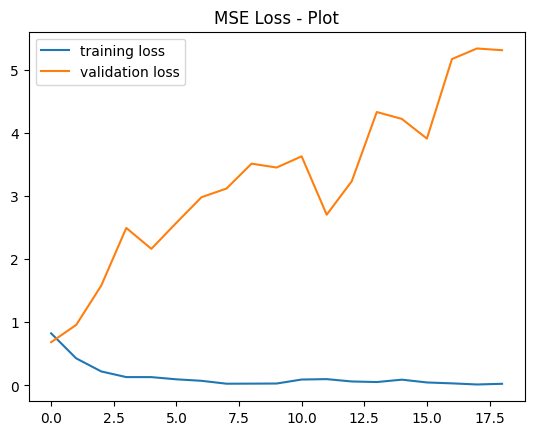
\includegraphics[width=\linewidth]{loss-no-transformer.png}
    \caption{non-LM-based classifier cross entropy loss.}
    \label{fig:1}
\end{figure}
	
\begin{figure}
    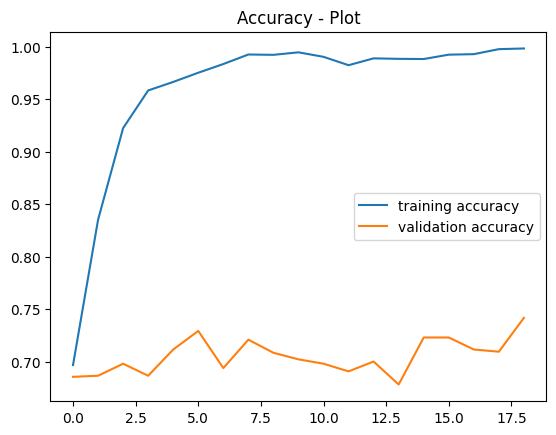
\includegraphics[width=\linewidth]{accuracy-no-transformer.png}
    \caption{non-LM-based classifier accuracy.}
    \label{fig:2}
\end{figure}
	
\begin{figure}
    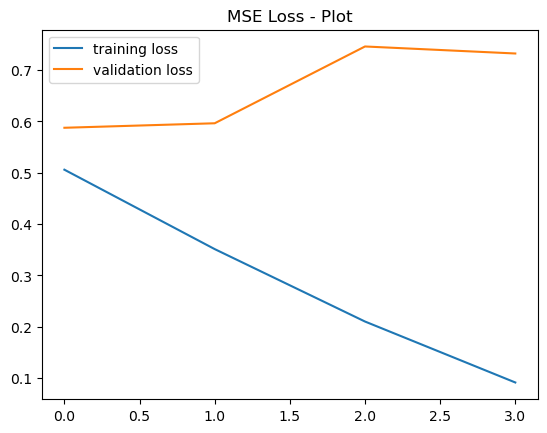
\includegraphics[width=\linewidth]{loss-yes-transformer.png}
    \caption{LM-based classifier cross entropy loss.}
    \label{fig:3}
\end{figure}
	
\begin{figure}
    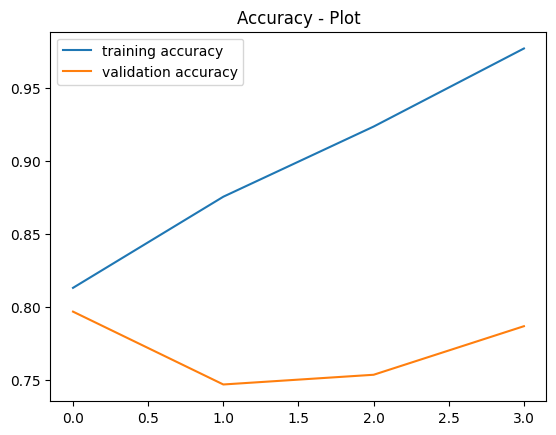
\includegraphics[width=\linewidth]{accuracy-yes-transformer.png}
    \caption{LM-based classifier accuracy.}
    \label{fig:4}
\end{figure}
	
\npdecimalsign{.}
\nprounddigits{3}
	
\begin{table}[]
    \small
    \caption{non-LM-based classifier training}
    
    \begin{tabular}{n{4}{2}|n{4}{2}|n{4}{2}|n{4}{2}}
        \toprule
	\multicolumn{1}{|l|}{train\_loss} & \multicolumn{1}{l|}{train\_accuracy} & \multicolumn{1}{l|}{valid\_loss} & \multicolumn{1}{l|}{valid\_accuracy} \\ \midrule
			0.824580834836376 & 0.6966198980808258 & 0.6848233610391616 & 0.6854166686534882 \\
			0.42828274567668534 & 0.8351084182457048 & 0.958229947090149 & 0.6864583313465118 \\
			0.22107240875080533 & 0.9225127551020408 & 1.5812558472156524 & 0.6979166686534881 \\
			0.13131998874406253 & 0.9583864795918368 & 2.4951072216033934 & 0.6864583313465118 \\
			0.130913822639945 & 0.9665178571428571 & 2.16357661485672 & 0.7114583313465118 \\
			0.09606347653952609 & 0.9752869897959183 & 2.5771642506122587 & 0.7291666686534881 \\
			0.07248458779450834 & 0.9835778061224489 & 2.981712055206299 & 0.69375 \\
			0.0265690988670643 & 0.9926658163265306 & 3.1195664286613463 & 0.7208333313465118 \\
			0.027661062501474775 & 0.9923469387755102 & 3.513991141319275 & 0.7083333313465119 \\
			0.029358040371947454 & 0.9947385204081632 & 3.4526482462882995 & 0.7020833313465118 \\
			0.09277717625173186 & 0.9904336734693877 & 3.629844832420349 & 0.6979166686534881 \\
			0.09905036353343255 & 0.9824617346938775 & 2.7048511862754823 & 0.690625 \\
			0.061935576511582345 & 0.9889987244897959 & 3.2353042364120483 & 0.7 \\
			0.05289996036179552 & 0.9885204081632653 & 4.332302975654602 & 0.678125 \\
			0.0905823381769124 & 0.9883609693877551 & 4.223013067245484 & 0.7229166686534881 \\
			0.04633352841285057 & 0.9925063775510204 & 3.9111754536628722 & 0.7229166686534881 \\
			0.03198182235851616 & 0.9929846938775511 & 5.171815228462219 & 0.7114583313465118 \\
			0.014295995866217713 & 0.9977678571428571 & 5.33933527469635 & 0.709375 \\
			0.02501944363913569 & 0.998405612244898 & 5.311948704719543 & 0.7416666686534882 \\
			\cmidrule(r){1-4}
    \end{tabular}
    \label{table:1}
\end{table}
	
\begin{table}[]
    \caption{LM-based classifier training}
	\begin{tabular}{n{4}{2}|n{4}{2}|n{4}{2}}
		\toprule
			\multicolumn{1}{|l|}{train\_loss} & \multicolumn{1}{l|}{valid\_loss} & \multicolumn{1}{l|}{valid\_accuracy} \\ \midrule
			null & 0.547339 & 0.796667 \\
			null & 0.569936 & 0.746667 \\
			0.571500 & 0.661266 & 0.753333 \\
			0.571500 & 0.730450 & 0.786667 \\
			\cmidrule(r){1-3}
	\end{tabular}
    \label{table:2}
\end{table}
	
\npnoround
	
Figures \ref{fig:1}, \ref{fig:2}, \ref{fig:3}, \ref{fig:4} and Tables \ref{table:1}, \ref{table:2} present the cross entropy
	loss and accuracy for each epoch during the training phases of the two models.
	
\section{Tested encoder models Appendix}
\label{sec:appendix2}
\begin{table}[]
		\small
		\caption{LM-based classifier training}
		\begin{tabular}{@{}l|lll@{}}
			\toprule
			& \multicolumn{1}{l|}{batch\_size} & \multicolumn{1}{l|}{epochs} & \multicolumn{1}{l|}{length} \\ \midrule
			\multicolumn{1}{|l|}{bigbird-roberta-base} & 4                                & 4                           & 4096                             \\ \cmidrule(r){1-1}
			\multicolumn{1}{|l|}{distilbert-base-uncased}     & 32                               & 30                          & 512                              \\ \cmidrule(r){1-1}
			\multicolumn{1}{|l|}{roberta-base}                & 32                               & 30                          & 512                              \\ 
			\cmidrule(r){1-1}
			\multicolumn{1}{|l|}{roberta-large}                & 32                               & 30                          & 512                              \\ 
			\cmidrule(r){1-1}
			\multicolumn{1}{|l|}{xlm-roberta-base}            & 32                               & 30                          & 512                              \\ \cmidrule(r){1-1}
			\multicolumn{1}{|l|}{xlm-roberta-large}           & 32                               & 30                          & 512                              \\ \cmidrule(r){1-1}
			\multicolumn{1}{|l|}{mdeberta-v3-base}  & 32                               & 30                          & 512                              \\ \cmidrule(r){1-1}
			\multicolumn{1}{|l|}{mdeberta-v3-large} & 32                               & 30                          & 512                              \\ \bottomrule
		\end{tabular}
		\label{table:3}
	\end{table}
	
	Table \ref{table:3} lists the base encoder models we tested for the LM-based classifier. We selected RoBERTa-base based on a trade-off between performance and validation set accuracy. For instance, some models—such as BigBird—are too large to run efficiently on standard machines with typical GPUs.

	\section{File description Appendix}
	\label{sec:appendix}
	
	In this section we will describe the content of the \href{https://drive.google.com/drive/folders/1t5pgHkdenMFPdKqQweiFl8vhIAaiVFTM?usp=drive_link}{shared Google drive directory}.
	
	\subsection{Colab(s)}
	
	\emph{NLP\_no\_transformer\_training.ipynb}: non-LM-based training Colab, the trained model is pushed to the
	\href{https://huggingface.co/fax4ever/culturalitems-no-transformer}{Hugging Face repo for non-LM-based}.
	
	\noindent \emph{NLP\_no\_transformer\_inference.ipynb}: non-LM-based inference Colab, the trained model is pulled from the
	\href{https://huggingface.co/fax4ever/culturalitems-no-transformer}{Hugging Face repo for non-LM-based}.
	
	\noindent \emph{NLP\_yes\_transformer\_training.ipynb}: LM-based training Colab, the trained model is pushed to the
	\href{https://huggingface.co/fax4ever/culturalitems-roberta-base}{Hugging Face repo for LM-based}.
	
	\noindent \emph{NLP\_no\_transformer\_inference.ipynb}: LM-based inference Colab, the trained model is pulled from the
	\href{https://huggingface.co/fax4ever/culturalitems-roberta-base}{Hugging Face repo for LM-based}.
	
	\subsection{Data loaded dumps}

	These dumps contain data retrieved from Wikipedia pages and Wikidata entities online. 
	Since this content is mutable, results may vary if the files are regenerated. 
	If you want to reproduce the exact results described in the report, please use these files. 
	Remove them if your goal is to test the Colab’s ability to generate them from scratch:
	
	 \begin{itemize}
	 	\item training.bin
	 	\item validation.bin
	 	\item test.bin
	 \end{itemize}
	 
	 \subsection{Processed data dumps}
	 
	 These are used only by the non-LM-based components. Unlike the others, 
	 they can be safely deleted without affecting the results, 
	 as they simply store preprocessed data derived from the original sources. 
	 Use them to speed up training and inference. 
	 Remove them if your goal is to test Colab’s ability to recreate them:
	 
	 \begin{itemize}
	 	\item training-proc.bin
	 	\item validation-proc.bin
	 	\item test-proc.bin
	 \end{itemize}
	
	\subsection{Other files}
	
	\emph{Lost\_in\_Language\_Recognition\_output\_multimodalnn.csv}: non-LM-based inference result on the test set
	\emph{Lost\_in\_Language\_Recognition\_output\_roberta.csv}: LM-based inference result on the test set
	\emph{nlp-homework-1.pdf}: this report
	
	\section{Algorithms  Appendix}
	\label{sec:appendix}
	
	In this section we present some implementation ideas of the project, providing some
	code samples and describing them.
	
	\subsection{Pushing and Pulling Models from Hugging Face Repositories}
	
	For the LM-based component, we used Hugging Face’s Transformers high-level API. By using \emph{AutoModelForSequenceClassification}  the model instance provides a convenient 
	\emph{push\_to\_hub()} method for uploading the model to the Hugging Face Hub:
	
	\small
	\begin{lstlisting}[language=python]
model.push_to_hub(repo, token=...)
	\end{lstlisting}
	\normalsize
To load the fine-tuned model, we simply use \emph{AutoModelForSequenceClassification.from\_pretrained}. \newline Interestingly, we found that a similar workflow is possible even when using the lower-level PyTorch API, which we applied in the non-LM-based part. This requires the model class to extend the \emph{PyTorchModelHubMixin} interface. \newline A few guidelines must be followed. For instance, all constructor parameters need to be serializable. Additionally, to ensure the model can be reused seamlessly on both CPU and CUDA devices, we recommend not passing the device type to the constructor. Instead, provide a method within the model to set the device for its components. You can refer to the  \emph{MultiModalModel} class used in the non-LM-based implementation as an example. \newline The value of deploying the model to the Hub is that it becomes immutable and can be easily shared and tested across different environments.
	
\subsection{non-LM-based model}
The Wikidata description is used to generate two inputs for the model: a frequency vector based on a dictionary limited to 4,000 items, and a 20-word GloVe embedding, with each word represented by a 100-dimensional vector. The Wikipedia text is used separately to produce a frequency vector based on a different dictionary of 10,000 items. Additionally, for each entity, we collect a set of language indicators: those used in labels, descriptions, aliases, and Wikipedia pages. Since these sets share the same domain—the complete set of supported languages—we use a common dictionary to generate their corresponding frequency vectors. \newline For the properties (Wikidata claims of the entity), we chose to collect only the claim keys, which are then used to generate a frequency vector based on a separate dictionary. Additionally, we map the entity type and its category/subcategory, representing each as scalar values. The method used to compute the category/subcategory scalar values is described in the next subsection of the appendix. \newline As mentioned earlier, each of these inputs is rescaled using a dedicated mini-network, defined as follows:
\scriptsize
	\begin{lstlisting}[language=python]
return nn.Sequential(nn.Linear(inf, outf), nn.ReLU())
	\end{lstlisting}
\normalsize
This setup not only rescales each input into an embedding—whose size becomes a tunable hyperparameter—but also applies a non-linear activation function to the output. \newline In the forward method the result of all the inputs is concatenated using the \emph{torch.cat} function and passed to the classifier:
\scriptsize
	 \begin{lstlisting}[language=python]
combined = torch.cat([desc_feat, desc_glove_feat, 
  wiki_feat, labels_feat, descriptions_feat, 
  aliases_feat, pages_feat,
  claims_feat, category_feat, type_feat], dim=1)
return self.classifier(combined)
	 \end{lstlisting}
\normalsize
While the classifier is a very common FF network:
\scriptsize
    \begin{lstlisting}[language=python]
self.classifier = nn.Sequential(
  nn.Linear(params['total_scale'],  params['hidden_layers']),
  nn.ReLU(),
  nn.Dropout(params['dropout']),
  nn.Linear(params['hidden_layers'], 3)
)
    \end{lstlisting}
\normalsize
	 
\subsection{Production of the Category/Subcategory Scalar}
Instead of mapping each category and subcategory to separate scalar values, we leveraged the fact that each subcategory uniquely determines its category. Using the Pandas library, we first collect all category–subcategory pairs. We then sort them by category so that subcategories belonging to the same category appear adjacent in the resulting ID sequence:
\scriptsize
	\begin{lstlisting}[language=python]	
def build(self):
  data = {
    'subcategory': self.subcategories,
    'category': self.categories
  }
  df = pd.DataFrame(data)
  df = df.sort_values('category')
  print(df.to_markdown())
  self.subcategory_to_id = {row["subcategory"]: 
    index for index, (_, row) in enumerate(df.iterrows())}

def subcat_to_vector(self, subcategory):
  vector = np.zeros(1, dtype=np.float32)
  vector[0] = vector[0] + self.subcategory_to_id[subcategory]
  return vector
	\end{lstlisting}
\normalsize
With this approach, a single scalar value encodes both the subcategory (directly as its ID) and the category (implicitly as a range of adjacent IDs). According to our experiments, this design improves classification performance.
	
\section{Team specialization Appendix}
\label{sec:appendix}
Significant work on hyperparameter optimization was carried out by Nicolò Della Porta, who, for example, extensively explored and applied \href{https://optuna.org/}{Optuna}  for this purpose across both the non-LM-based and LM-based models. Giovanni Regina focused on identifying domain-specific heuristic rules to generate additional features, helping to enhance the classifier’s performance in both model types. Fabio Massimo Ercoli concentrated more on the non-LM-based model, particularly contributing to the design and implementation of input rescaling strategies and the category scalar idea.
\end{document}

